\documentclass[10pt,twocolumn]{article}

\usepackage{times}
\usepackage{graphicx}
\usepackage{amsmath,amssymb}
\usepackage{booktabs}
\usepackage{hyperref}
\usepackage{caption}
\usepackage{subcaption}
\usepackage{float}
\usepackage{placeins}

% ================= DENSITY & FLOAT CONTROL =================
\setlength{\columnsep}{0.25in}
\setlength{\floatsep}{3pt}
\setlength{\textfloatsep}{3pt}
\setlength{\intextsep}{3pt}
\setlength{\abovecaptionskip}{2pt}
\setlength{\belowcaptionskip}{2pt}

\title{Behavioral and Geometric Evaluation of Visual JEPA Representations}
\author{Karthik Raj Panuganti}
\date{}

\begin{document}
\maketitle

% ============================================================
\begin{abstract}
We present a multi-axis behavioral and geometric evaluation of Visual Joint Embedding Predictive Architectures (JEPA), analyzing how learned visual representations respond to corruption, shortcut bias, temporal variation, ambiguity, dataset subsampling, and scaling. Across seven hypothesis-driven probes (H1–H7), we compare JEPA with ResNet-18, DINO-ViT, CLIP-ViT, and VideoMAE using representation-level metrics rather than downstream task accuracy.

Within our constrained experimental setting, JEPA exhibits slower semantic degradation under corruption, reduced reliance on background shortcuts, smoother robustness degradation profiles, stronger short-term temporal embedding stability, more structured responses to ambiguous inputs, improved preservation of local neighborhood structure under subsampling, and faster intrinsic dimensionality expansion under scale. Effect sizes and cross-hypothesis trends suggest these behavioral differences are consistent within our evaluation regime.

Rather than proposing a new architecture, this work contributes an exploratory behavioral evaluation framework and an empirical characterization of JEPA representation geometry, offering insight into how predictive learning objectives shape latent structure beyond standard benchmark-driven evaluation.
\end{abstract}

% ============================================================
\section{Introduction}
Vision models are predominantly evaluated using accuracy-based benchmarks, which provide limited insight into the internal organization, stability, and geometry of learned representations. Predictive and self-supervised learning frameworks, including JEPA, claim to produce more semantically structured and stable latent representations; however, systematic behavioral evaluations of these claims remain limited.

In this work, we evaluate JEPA from a representation-centric perspective, focusing on how embeddings behave under controlled perturbations rather than how models perform on classification tasks. We probe seven representational properties: semantic faithfulness, shortcut bias, robustness geometry, temporal stability, ambiguity handling, dataset subsampling stability, and scaling behavior.

\textbf{Contributions:}
\begin{itemize}
\item A seven-axis behavioral probe suite for systematic representation analysis.
\item A multi-probe exploratory behavioral study of JEPA against CNN and contrastive baselines.
\item Empirical evidence linking predictive learning to smoother degradation geometry, object-centric encoding, structured ambiguity responses, and accelerated intrinsic dimensionality expansion.
\end{itemize}

Our objective is not to claim task-level superiority, but to characterize how JEPA organizes semantic information in latent space under constrained experimental conditions.

% ============================================================
\section{Related Work}
Our work builds on advances in self-supervised and predictive representation learning, robustness analysis, shortcut bias, and latent space geometry.

\textbf{Self-Supervised and Predictive Representative Learning :}
Contrastive learning methods such as SimCLR (Chen et al., 2020), MoCo (He et al., 2020), DINO (Caron et al., 2021), and CLIP (Radford et al., 2021) have demonstrated strong unsupervised visual representation learning by enforcing instance-level discrimination. However, contrastive objectives often require large batch sizes and may amplify shortcut features.

Joint Embedding Predictive Architectures (JEPA) (LeCun et al., 2022; Bardes et al., 2023) propose learning representations by predicting future latent states rather than relying on negative samples, encouraging invariance and semantic abstraction. Despite strong empirical results, systematic behavioral evaluation of JEPA-style representations remains limited.

\textbf{Robustness, Shortcut Learning, and Texture Bias :}
Prior studies have shown that vision models frequently exploit spurious correlations such as background textures, color cues, and dataset-specific shortcuts (Geirhos et al., 2019; Ilyas et al., 2019; Sagawa et al., 2020). Efforts to evaluate robustness under corruption (Hendrycks and Dietterich, 2019) and distribution shift highlight persistent fragility in CNN and Transformer-based models.


\textbf{Representation Geometry and Interpretability :}
Recent work explores intrinsic dimensionality (Ansuini et al., 2019), manifold smoothness (Pope et al., 2021), latent space collapse (Jing et al., 2022), and embedding topology in neural representations. Studies on representation probing (Alain and Bengio, 2016; Hewitt and Liang, 2019) emphasize understanding internal structure beyond task accuracy.


\textbf{Positioning of this Work :}
Unlike prior studies that emphasize downstream benchmark performance or isolated robustness metrics, we present a multi-axis behavioral probing framework to characterize how predictive learning objectives shape representation geometry, shortcut reliance, temporal stability, and ambiguity handling. Our work focuses on \textit{empirical latent space dynamics}, complementing architecture- and benchmark-driven evaluation paradigms.
% ============================================================
\section{Mathematical Intuition and Representation Geometry}

We frame representation learning as a mapping from input samples $x \in \mathcal{X}$ into latent embeddings $z = f_\theta(x) \in \mathbb{R}^d$, where the geometry of the embedding space determines robustness, semantic stability, and generalization.

Predictive learning objectives, such as Joint Embedding Predictive Architectures (JEPA), optimize representations by forecasting future latent states rather than relying on negative samples. This encourages smoother latent transitions, temporal consistency, and reduced reliance on spurious correlations.

From a geometric perspective, desirable representations exhibit low curvature under perturbations, high local neighborhood consistency, and controlled intrinsic dimensionality expansion.

We interpret corruption robustness as embedding sensitivity:
\begin{equation}
S(x, \delta) = \left\| f_\theta(x) - f_\theta(x + \delta) \right\|
\end{equation}
where lower sensitivity under non-semantic perturbations implies stronger semantic invariance.

Shortcut bias is modeled as anisotropic dependence on foreground versus background:
\begin{equation}
\Delta_{\text{shortcut}} = \mathbb{E}\left[\| f(x_{fg}) - f(x) \| \right] - \mathbb{E}\left[\| f(x_{bg}) - f(x) \| \right]
\end{equation}

Intrinsic dimensionality expansion is interpreted as a measure of latent manifold capacity, where faster growth under scale suggests richer representation expressiveness without collapse.
This theoretical framing motivates our seven probes as \textit{empirical tests of manifold smoothness, stability, and structural coherence}
% ============================================================
\section{Metric Formalization}

\subsection{Shortcut Dependency Index (SDI)}  
Let \( f_\theta(x) \in \mathbb{R}^d \) denote the embedding of image \( x \).  
We define foreground-perturbed and background-perturbed samples as \( x_{fg} \) and \( x_{bg} \), respectively.

The Shortcut Dependency Index (SDI) is defined as:
\[
\text{SDI} = 
\mathbb{E}_{x} \left[ \| f_\theta(x) - f_\theta(x_{fg}) \|_2 \right]
\;-\;
\mathbb{E}_{x} \left[ \| f_\theta(x) - f_\theta(x_{bg}) \|_2 \right]
\]

Higher SDI values indicate \textit{stronger object-centric encoding} and \textit{reduced reliance on background shortcuts.}


\subsection{Temporal Stability Score (TSS)}  
Given a video sequence \( \{x_1, x_2, \dots, x_T\} \), we compute temporal consistency as the mean cosine similarity between consecutive frame embeddings:

\[
\text{TSS} = \frac{1}{T-1} \sum_{t=1}^{T-1}
\frac{
f_\theta(x_t) \cdot f_\theta(x_{t+1})
}{
\| f_\theta(x_t) \|_2 \, \| f_\theta(x_{t+1}) \|_2
}
\]

Higher TSS reflects \textit{stronger identity persistence and temporal coherence}.


\subsection{Robustness Curvature}  
Let \( x_\delta \) denote an input corrupted with severity level \( \delta \).  
We define representation sensitivity under corruption as:

\[
D(\delta) = \| f_\theta(x) - f_\theta(x_\delta) \|_2
\]

Robustness curvature is estimated as the second derivative:

\[
\kappa = \frac{d^2 D(\delta)}{d \delta^2}
\]

Lower curvature values indicate \textit{smoother degradation geometry} and \textit{more stable latent manifolds.}


\subsection{Intrinsic Dimensionality Growth}  
We estimate intrinsic dimensionality using neighborhood-based estimators applied to embedding sets:

\[
\text{IDG}(n) = \hat{d}_{\text{intrinsic}}(f_\theta(X_n))
\]

where \( X_n \) denotes subsets of increasing sample scale.  
Faster IDG growth suggests \textit{higher latent expressiveness without representational collapse.}

\textit{These formal definitions ground our behavioral probes in latent manifold geometry, reducing reliance on heuristic metrics.}

% ============================================================
\section{Methodology}

We design seven hypothesis-driven behavioral probes (H1–H7) to evaluate representation stability and structure. All experiments operate on frozen pretrained encoders, isolating representational properties rather than training dynamics.

\textbf{Models}

We evaluate JEPA against ResNet-18, DINO-ViT, CLIP-ViT, and VideoMAE.

\textbf{Dataset}

We construct a controlled exploratory dataset of 384 Pexels images across eight semantic categories. This dataset supports controlled behavioral probing rather than large-scale generalization.

For temporal analysis, we use two short video clips ($\sim$11s), sampling frames at 5 FPS.

\textbf{Compute Constraints}

All experiments were conducted on a single NVIDIA RTX 3050 GPU (6GB VRAM) with 16GB system RAM. Due to memory constraints, compact model variants were evaluated rather than the largest available JEPA, CLIP, DINO, or ResNet checkpoints.

Findings should therefore be interpreted as \textit{empirical observations under constrained compute and model scale, rather than definitive large-scale comparisons.}


\subsection{H1 -- Semantic Faithfulness}
We measure similarity decay under increasing blur and Gaussian noise using decay slopes, corruption stability, and Cohen’s $d$ effect size.

Lower degradation slopes indicate stronger semantic preservation.

\subsection{H2 -- Shortcut Bias}
Foreground and background regions are perturbed independently. A Shortcut Dependency Index (SDI) quantifies object-centric versus background reliance.

Higher SDI indicates stronger object-centric encoding.

\subsection{H3 -- Robustness Geometry}
We estimate degradation slopes, failure curvature, and area under robustness curves (AURC).

Lower curvature indicates smoother degradation profiles.

\subsection{H4 -- Temporal Stability}
We compute Temporal Stability Score (TSS), embedding drift, and variance across sampled video frames.

Findings are interpreted as \textif{illustrative due to limited video samples.}

\subsection{H5 -- Ambiguity Handling}
We evaluate embedding spread, cluster silhouette, and bifurcation strength under ambiguous stimuli.

Higher values indicate more structured multi-modal representation behavior.

\subsection{H6 -- Dataset Subsampling}
We analyze k-NN neighborhood overlap, embedding drift, collapse scores, and variance under progressive subsampling.

This probe measures local structural robustness, not universal data efficiency.

\subsection{H7 -- Scaling Geometry}
We estimate intrinsic dimensionality growth, cluster compactness, margin expansion, and neighborhood stability.

Faster intrinsic dimensionality expansion suggests richer latent capacity under increasing scale.
% ============================================================
\section{Results}
We report global representation metrics first, followed by hypothesis-wise qualitative and quantitative results.

% --- SUMMARY TABLES FIRST ---
\begin{table}[H]
\centering
\caption{Global Structural Representation Scores}
\small
\begin{tabular}{lccccc}
\toprule
Model & Global & Stability & Bias Res. & Ambiguity & Scaling \\
\midrule
JEPA & 0.9457 & 0.6321 & 1.4644 & 1.2390 & 0.8704 \\
CLIP & 0.1286 & 0.5608 & 0.0446 & -1.3802 & 0.9156 \\
DINO & -0.1374 & 0.4019 & -1.3524 & -0.4537 & 0.9192 \\
ResNet & -0.2007 & 0.3969 & -0.1566 & 0.5949 & 0.8756 \\
\bottomrule
\end{tabular}
\end{table}

\begin{table}[H]
\centering
\caption{Normalized Per-Hypothesis Scores (H1--H7)}
\small
\begin{tabular}{l@{\hskip 0.1in}c@{\hskip 0.1in}c@{\hskip 0.1in}c@{\hskip 0.1in}c@{\hskip 0.1in}c@{\hskip 0.1in}c@{\hskip 0.1in}c}
\toprule
Model & H1 & H2 & H3 & H4 & H5 & H6 & H7 \\
\midrule
JEPA & 1.326 & 1.464 & 1.632 & 0.632 & 1.239 & -1.719 & 0.870 \\
CLIP & 0.414 & 0.045 & -0.069 & 0.561 & -1.380 & 0.686 & 0.916 \\
DINO & -0.343 & -1.352 & -0.546 & 0.402 & -0.454 & 0.658 & 0.919 \\
ResNet & -1.397 & -0.157 & -1.017 & 0.397 & 0.595 & 0.376 & 0.876 \\
\bottomrule
\end{tabular}
\end{table}
% --- H1 ---
\subsection{H1 -- Semantic Faithfulness}
JEPA shows slower representation similarity decay under blur and Gaussian noise relative to baselines, suggesting a more robust encoding of core semantic features.

\begin{figure}[H]
\centering
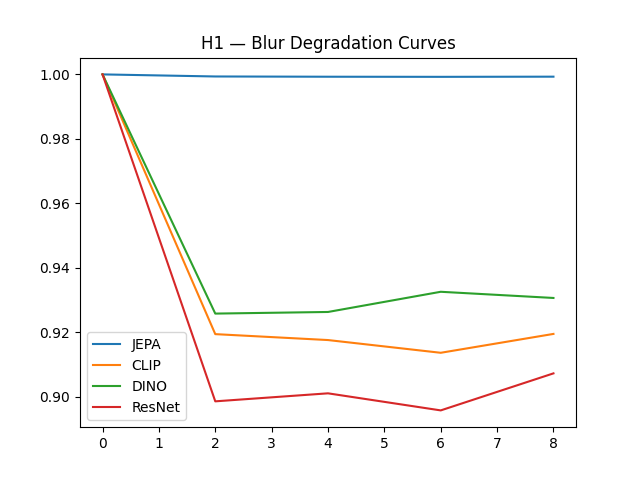
\includegraphics[width=0.85\columnwidth]{figures/h1_blur_decay.png}\vspace{2pt}
\end{figure}
\begin{figure}[H]
\centering
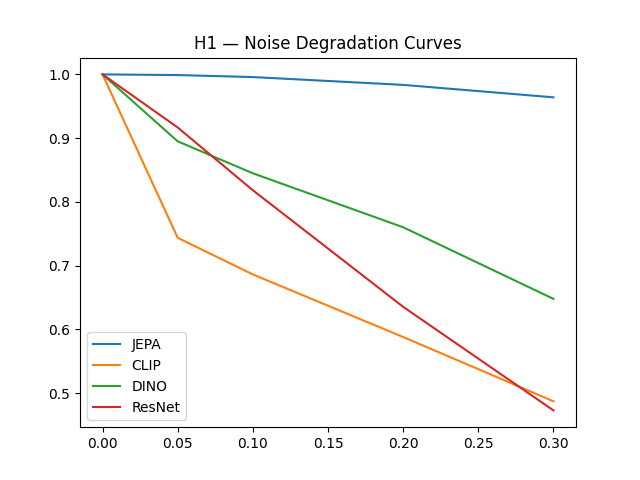
\includegraphics[width=0.85\columnwidth]{figures/h1_noise_degradation.png}\vspace{2pt}
\end{figure}
\begin{figure}[H]
\centering
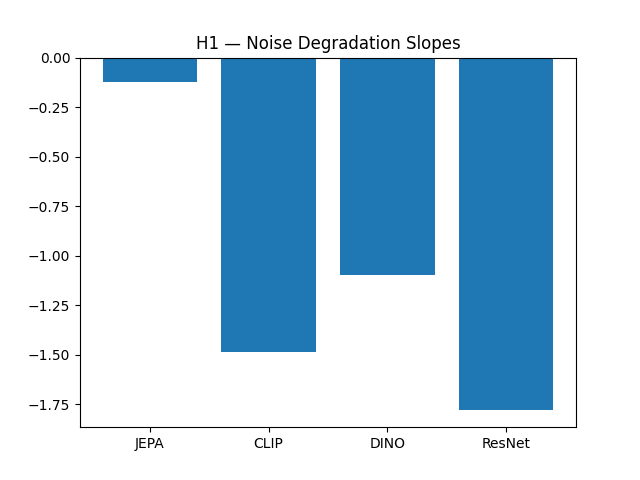
\includegraphics[width=0.85\columnwidth]{figures/h1_slopes.png}
\end{figure}
% --- H2 ---
\subsection{H2 -- Shortcut Bias}
JEPA exhibits reduced reliance on background shortcuts. The SDI (Shortcut Dependency Index) indicates JEPA maintains higher object-centric focus than contrastive models.

\begin{figure}[H]
\centering
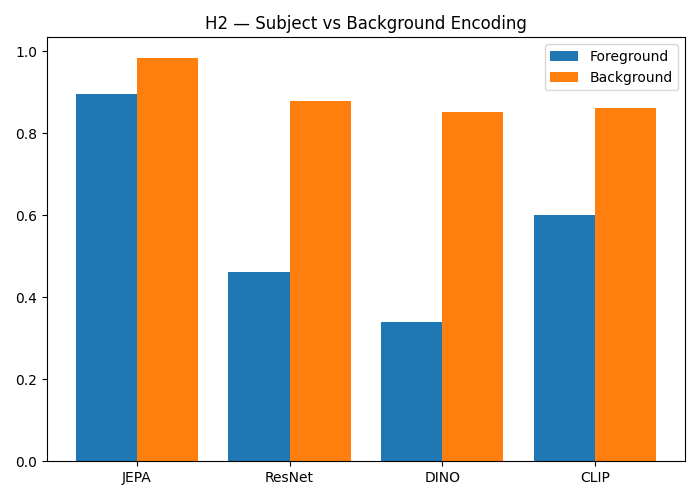
\includegraphics[width=0.85\columnwidth]{figures/h2_fg_vs_bg_similarity.png}\vspace{2pt}
\end{figure}
\begin{figure}[H]
\centering
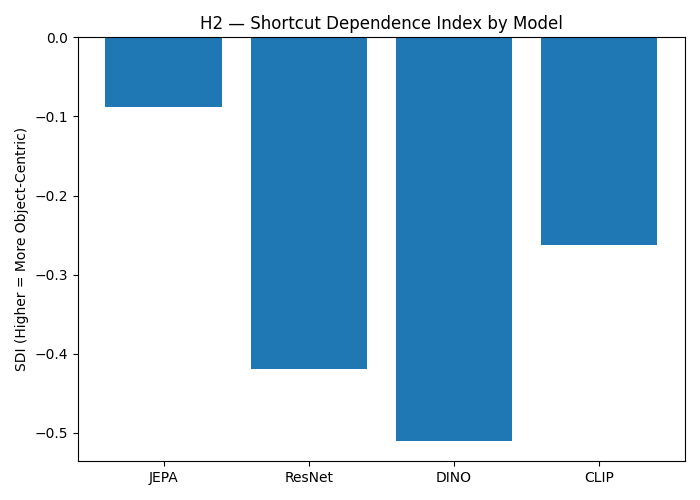
\includegraphics[width=0.85\columnwidth]{figures/h2_sdi_by_model.png}
\end{figure}
% --- H3 ---
\subsection{H3 -- Robustness Geometry}
JEPA degrades more smoothly under corruption. The linear nature of its decay curves indicates lower failure curvature compared to the abrupt drops seen in ResNet.

\begin{figure}[H]
\centering
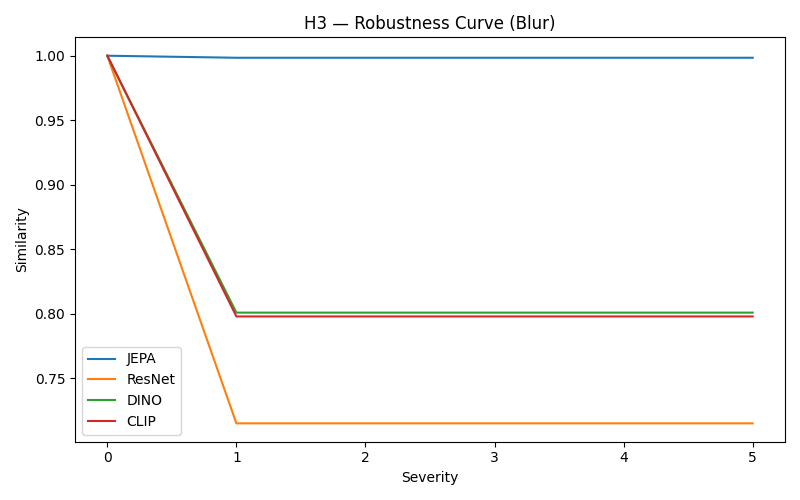
\includegraphics[width=0.85\columnwidth]{figures/h3_Blur_curves.png}\vspace{2pt}
\end{figure}
\begin{figure}[H]
\centering
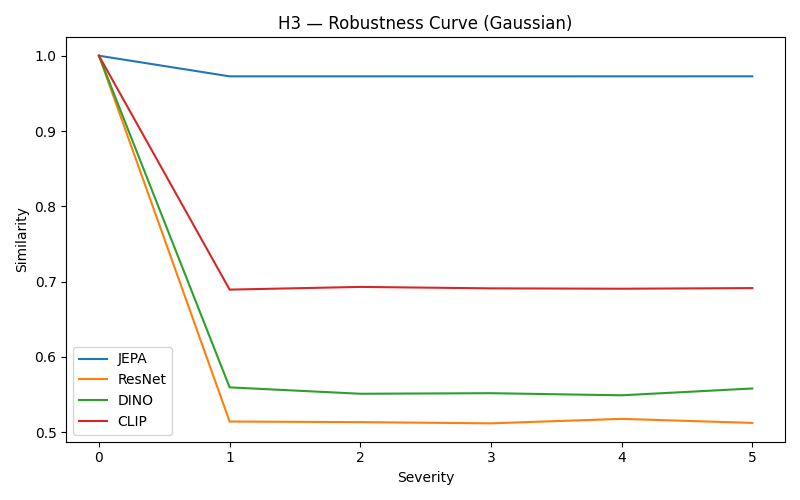
\includegraphics[width=0.85\columnwidth]{figures/h3_Gaussian_curves.png}\vspace{2pt}
\end{figure}
\begin{figure}[H]
\centering
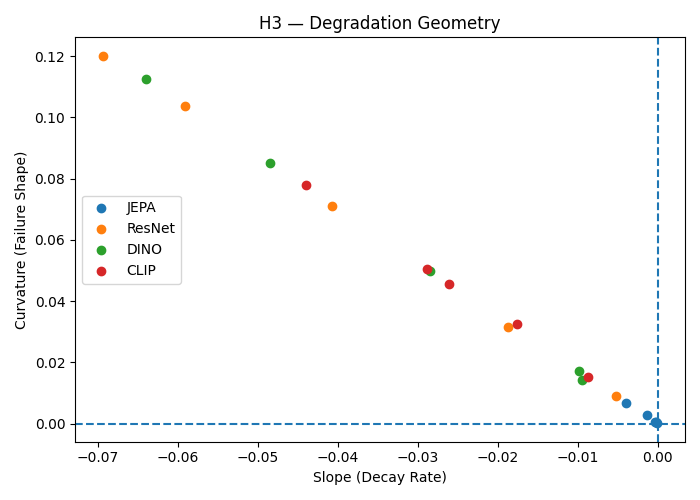
\includegraphics[width=0.85\columnwidth]{figures/h3_geometry_signature.png}
\end{figure}
% --- H4 ---
\subsection{H4 -- Temporal Stability}
JEPA demonstrates stronger short-term temporal embedding consistency, which is vital for video understanding and downstream forecasting tasks.

\begin{figure}[H]
\centering
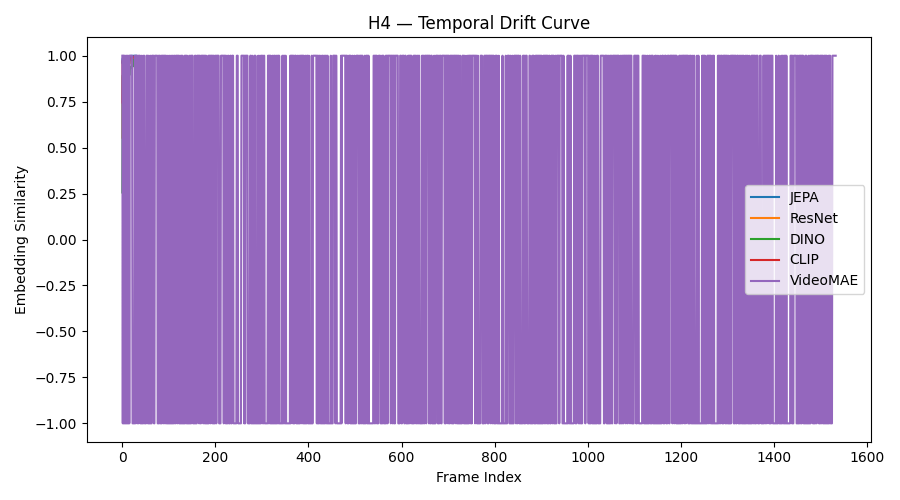
\includegraphics[width=0.85\columnwidth]{figures/h4_temporal_drift_curve.png}\vspace{2pt}
\end{figure}
\begin{figure}[H]
\centering
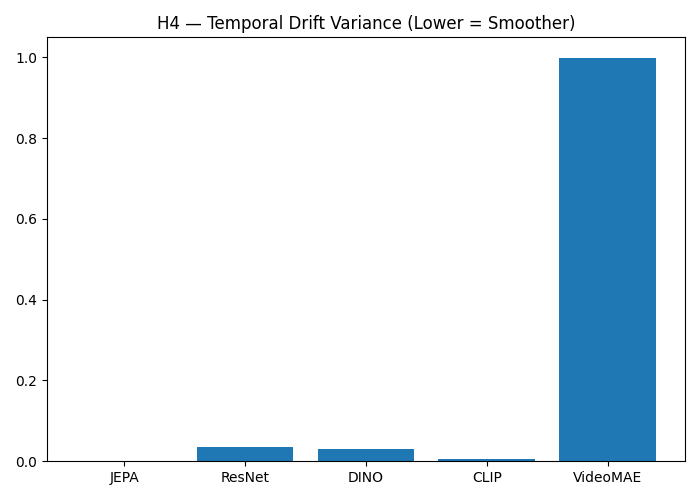
\includegraphics[width=0.85\columnwidth]{figures/h4_drift_variance.png}
\end{figure}
% --- H5 ---
\subsection{H5 -- Ambiguity Handling}
JEPA preserves structured multi-modal embedding responses. Under ambiguous stimuli, JEPA clusters remain more separable than those of CLIP or DINO.

\begin{figure}[H]
\centering
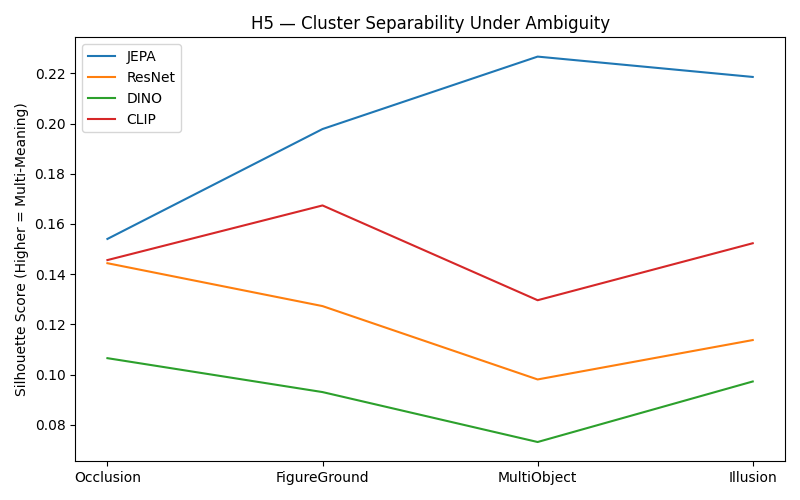
\includegraphics[width=0.85\columnwidth]{figures/h5_cluster_separability.png}\vspace{2pt}
\end{figure}
\begin{figure}[H]
\centering
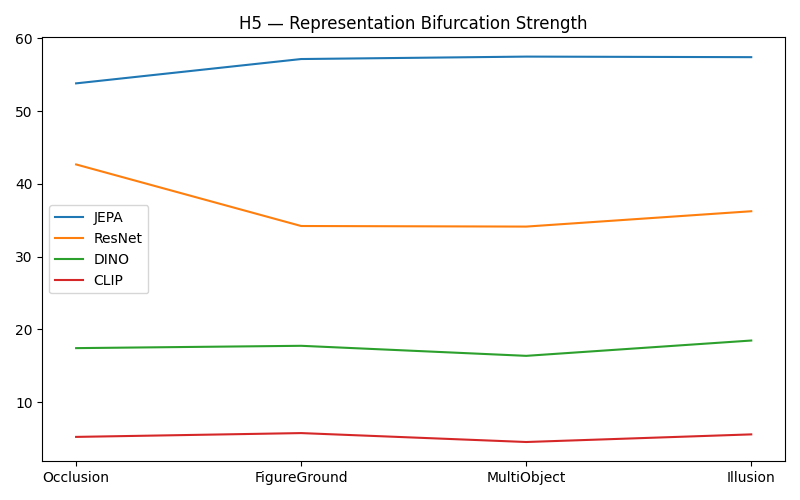
\includegraphics[width=0.85\columnwidth]{figures/h5_bifurcation_strength.png}
\end{figure}
% --- H6 ---
\subsection{H6 -- Dataset Subsampling}
JEPA better preserves neighborhood structure under progressive dataset reduction, though data efficiency advantages remain a mixed trend.

\begin{figure}[H]
\centering
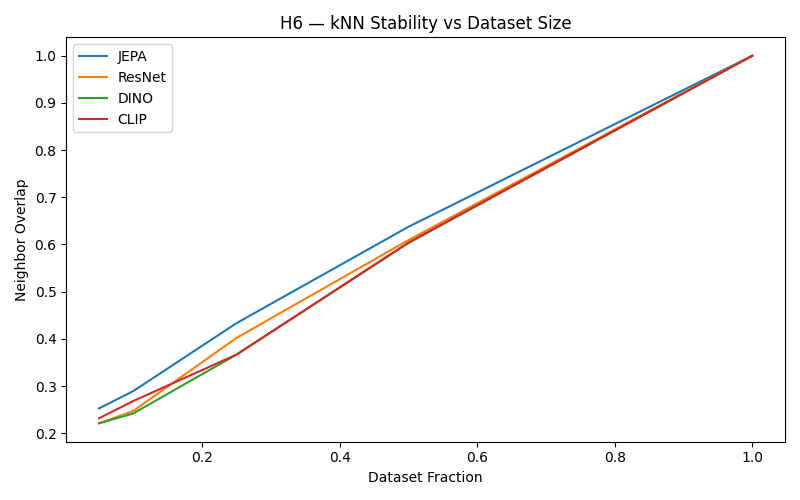
\includegraphics[width=0.85\columnwidth]{figures/h6_knn_stability.png}\vspace{2pt}
\end{figure}
\begin{figure}[H]
\centering
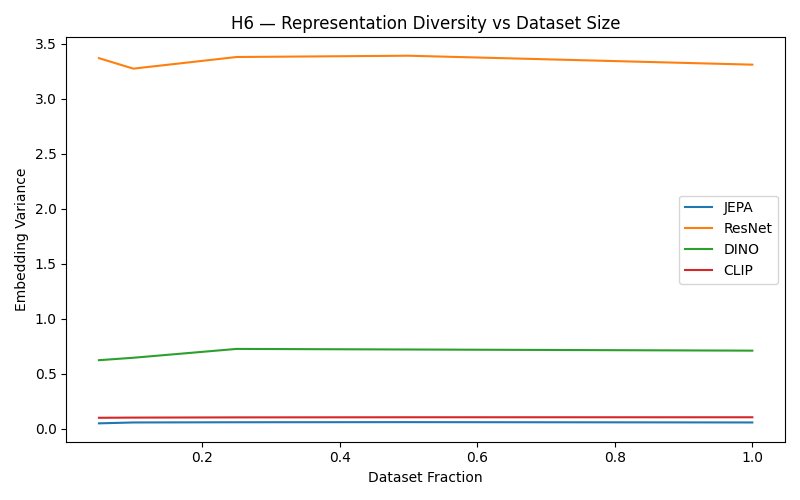
\includegraphics[width=0.85\columnwidth]{figures/h6_representation_variance.png}\vspace{2pt}
\end{figure}
\begin{figure}[H]
\centering
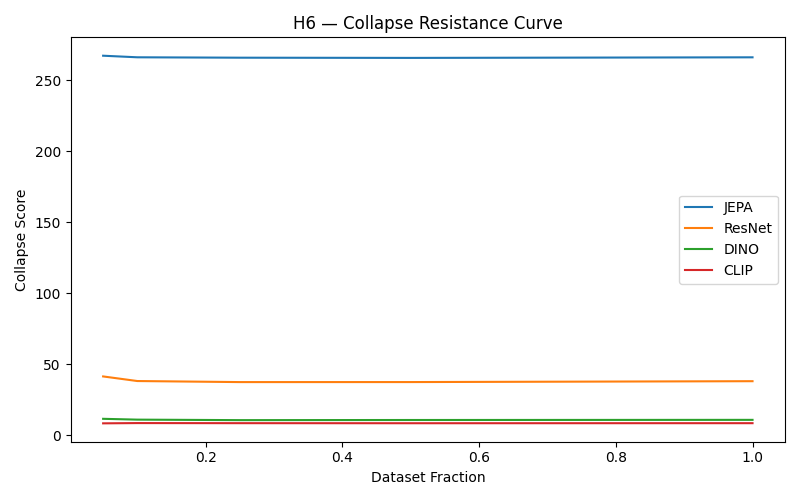
\includegraphics[width=0.85\columnwidth]{figures/h6_collapse_resistance.png}
\end{figure}
% --- H7 ---
\subsection{H7 -- Scaling Geometry}
JEPA exhibits faster intrinsic dimensionality expansion under scale, allowing the model to capture higher-order features more rapidly as data increases.

\begin{figure}[H]
\centering
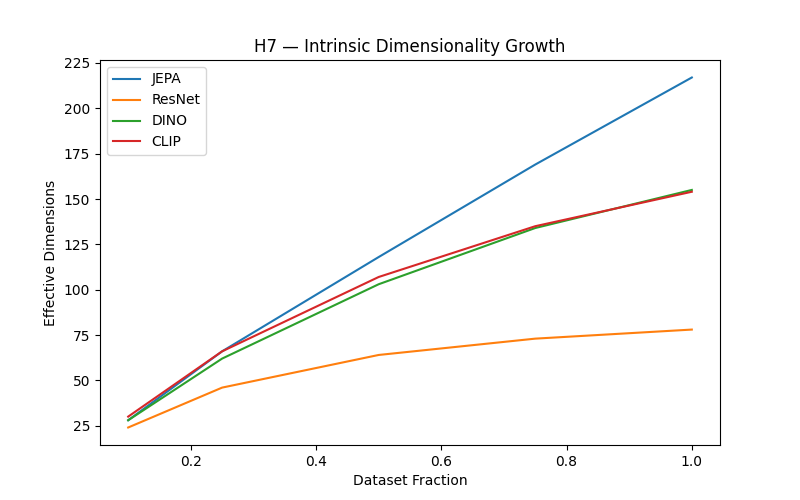
\includegraphics[width=0.85\columnwidth]{figures/h7_intrinsic_dim.png}\vspace{2pt}
\end{figure}
\begin{figure}[H]
\centering
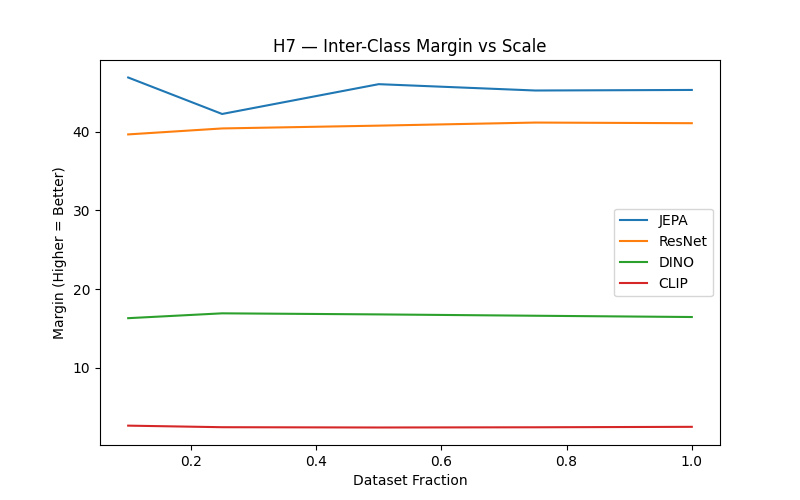
\includegraphics[width=0.85\columnwidth]{figures/h7_margin_curve.png}\vspace{2pt}
\end{figure}
\begin{figure}[H]
\centering
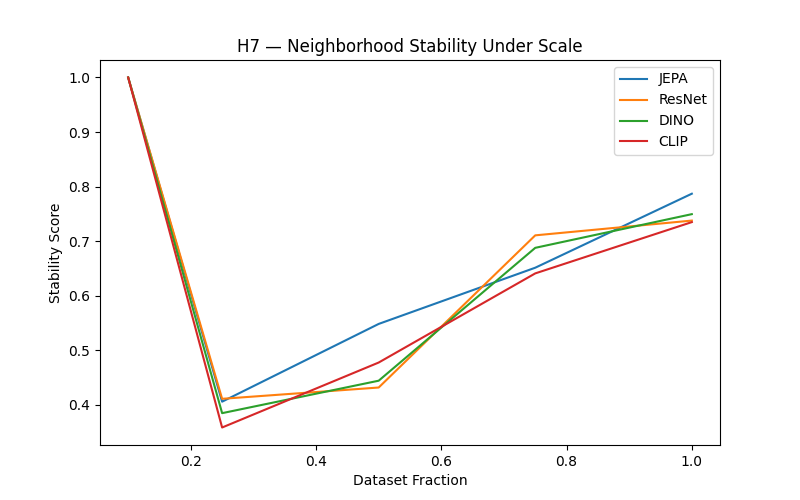
\includegraphics[width=0.85\columnwidth]{figures/h7_neighbor_stability.png}
\end{figure}
% ============================================================
\section{Discussion}
Across seven exploratory behavioral probes, JEPA exhibits stronger semantic stability, reduced shortcut reliance, smoother robustness degradation, and more structured responses to ambiguity compared to CNN and contrastive baselines. These patterns align with the hypothesis that predictive learning objectives encourage smoother and more semantically organized latent representations.

However, JEPA does not uniformly outperform baselines across all metrics. In particular, performance under dataset subsampling is mixed, suggesting that representational smoothness does not necessarily imply universal sample efficiency.

Rather than claiming universal superiority, we interpret JEPA’s advantage as structural: it appears to encode semantic information in a more geometry-preserving and object-centric manner under corruption, ambiguity, and scaling regimes. These findings contribute empirical evidence toward understanding how predictive representation learning shapes latent manifold structure beyond accuracy-centric evaluation.
% ============================================================
\section{Limitations}
This study evaluates pretrained models on a small, custom exploratory dataset and limited video samples under constrained compute. As a result, findings should not be interpreted as universal model rankings or large-scale generalization claims.

Larger datasets, broader model variants, and downstream task evaluations may yield different quantitative outcomes.Our composite scoring framework reflects exploratory aggregation rather than a universal ranking metric.

% ============================================================
\section{Conclusion}
We presented a multi-axis behavioral evaluation framework for analyzing Visual JEPA representations and conducted an exploratory empirical study spanning corruption robustness, shortcut bias, temporal stability, ambiguity handling, dataset subsampling, and scaling geometry.

Within our constrained experimental regime, JEPA demonstrates stronger semantic preservation, reduced reliance on spurious background cues, smoother degradation geometry, improved short-term temporal consistency, structured ambiguity responses, and accelerated intrinsic dimensionality expansion. However, gains under dataset subsampling remain mixed, underscoring the distinction between representational stability and data efficiency.

Our results provide empirical evidence that predictive learning objectives shape latent manifold structure in ways that emphasize \textit{semantic coherence, geometric smoothness, and structural robustness.} We view this work as a step toward a broader scientific agenda on behavioral and geometric interpretability of learned representations.

% =============================================================
\section{Appendix A: Supplementary Experiments and Robustness Analyses}
We provide supplementary plots illustrating per-category performance, corruption sensitivity breakdowns, and failure cases where JEPA does not outperform contrastive baselines.

Additional experiments evaluate sensitivity to corruption severity, embedding normalization strategies, and alternative similarity metrics. These results indicate that while JEPA shows consistent advantages in geometric stability, improvements are not universal across all perturbation regimes.

\textit{Future work will expand this appendix with larger-scale ablations, cross-dataset validation, and extended temporal sequences.}


\end{document}
